\section{QOC for the Fluxonium \label{sec:fluxonium}}
In the following, we optimize quantum gates
(unitary transformations) for the fluxonium qubit.
The fluxonium is a promising building block
for quantum computers, and the accurate
two-level approximation of its Hamiltonian makes
QOC on a classical computer inexpensive.
To high accuracy, we approximate the Hamiltonian near the flux frustration
as a spin-$1/2$ system:
\begin{align}
  H/h &= f_{q} \frac{\sigma_{z}}{2} + a(t) \frac{\sigma_{x}}{2},
  \label{eq:hamiltonian}
\end{align}
where $f_{q}$ is the qubit frequency at the flux frustration point,
$a(t)$ is the flux bias, $h$ is Planck's constant, and $\sigma_{z}, \sigma_{x}$
are Pauli matrices. Although we use an approximation for the Hamiltonian,
our noise model is realistic and considers the full Hilbert space. We optimize $X/2$,
$Y/2$, and $Z/2$ gates for the fluxonium presented in \cite{zhang2020universal},
and compare them to the analytically constructed gates for
that device.

First, we outline the constraints for the fluxonium gate problem.
We formulate this problem as a multi-state-transfer problem.
The initial conditions on
the states are $\ket{\psi^{0}_{1}} = \ket{0}$, $\ket{\psi^{1}_{1}} = \ket{1}$
\eqref{eq:istate_con}
where the superscript is an index $i \in \{0, 1\}$,
and the subscript indicates the first knot point $k = 1$.
The states at the final knot point are constrained to be
the image of the initial states under the desired gate $U$,
$\ket{\psi^{i}_{N}} = U \ket{\psi^{i}_{1}} \ \forall \ i$
\eqref{eq:tstate_con}.
Furthermore, we impose the normalization constraint
${\lvert \braket{\psi^{i}_{k}}{\psi^{i}_{k}} \rvert}^{2} = 1 \ \forall \ i,k$
\eqref{eq:statenorm_con}
to ensure the solver does not take advantage of discretization errors in numerical integration.
To refer to the discrete moments of the flux, we introduce the notation
$\int^{t_{k}}_{t_{1}} a(t) \ \mathrm{d}t \equiv \int_{t} a_{k}$,
$a(t = t_{k}) \equiv a_{k}$,
$\pdv*[n]{a(t)}{t} \lvert_{t = t_{k}} \equiv \partial^{n}_{t} a_{k}$.
We impose the zero net flux constraint $\int_{t} a_{N} = 0$
(seems kind of funny to be referencing the equations so far below - might be nicer to introduce the equations, referencing Eqs. (2)a-(2)d, then talk about what they mean.)
\eqref{eq:znf_con}
which mitigates the inductive drift ubiquitous in flux-bias lines
\cite{battistel2019fast, krantz2019quantum, zhang2020universal}.
The flux is constrained by $\lvert a_{k} \rvert \leq 0.5 \ \textrm{GHz} \ \forall \ k$
\eqref{eq:amp_con}
to ensure the two-level approximation \eqref{eq:hamiltonian} remains valid.
We also enforce the boundary condition $a_{1} = a_{N} = 0$ \eqref{eq:bound_con}
so the gates may be concatenated arbitrarily. Additionally,
we have the initial condition $\int_{t} a_{1} = \partial_{t} a_{1} = 0$
\eqref{eq:ic_con}.

%% F1
\begin{figure*}[ht]
  
  \begin{subfigure}{.315\textwidth}
    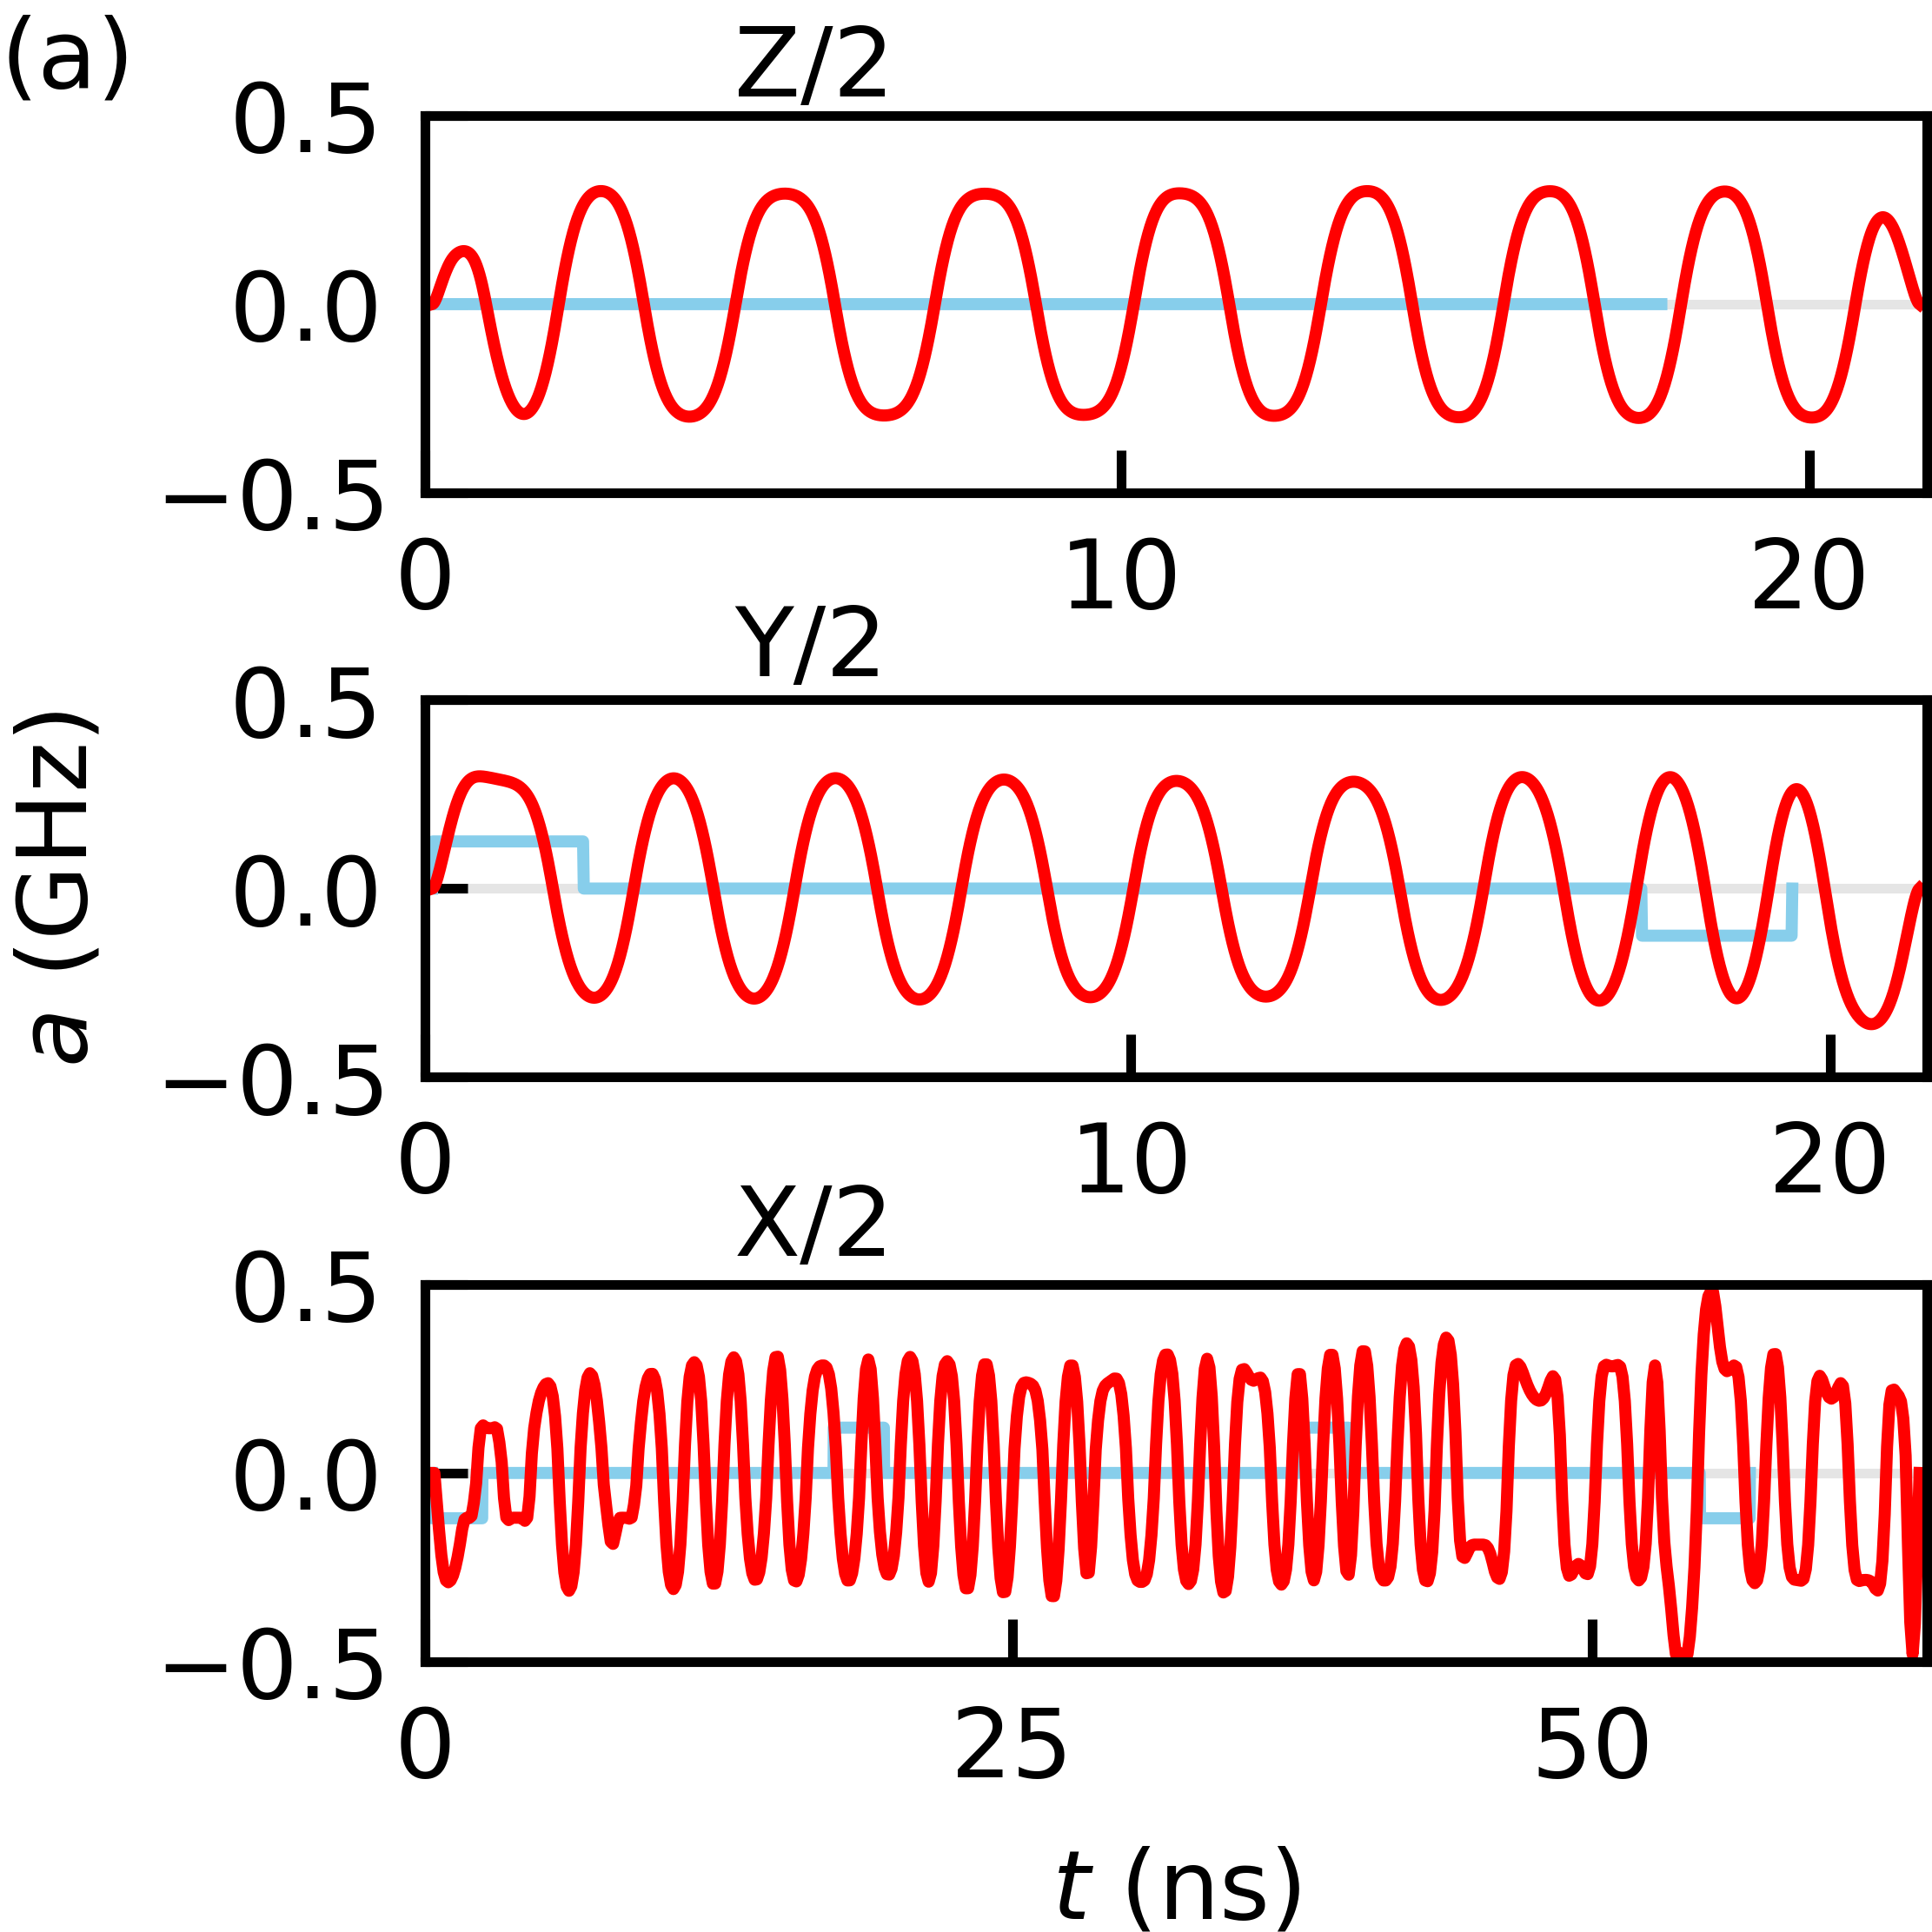
\includegraphics[width=\linewidth]{assets/f1a.png}
    \caption{\label{fig:longitudea}}
  \end{subfigure}\hfill
  \begin{subfigure}{.23\textwidth}
    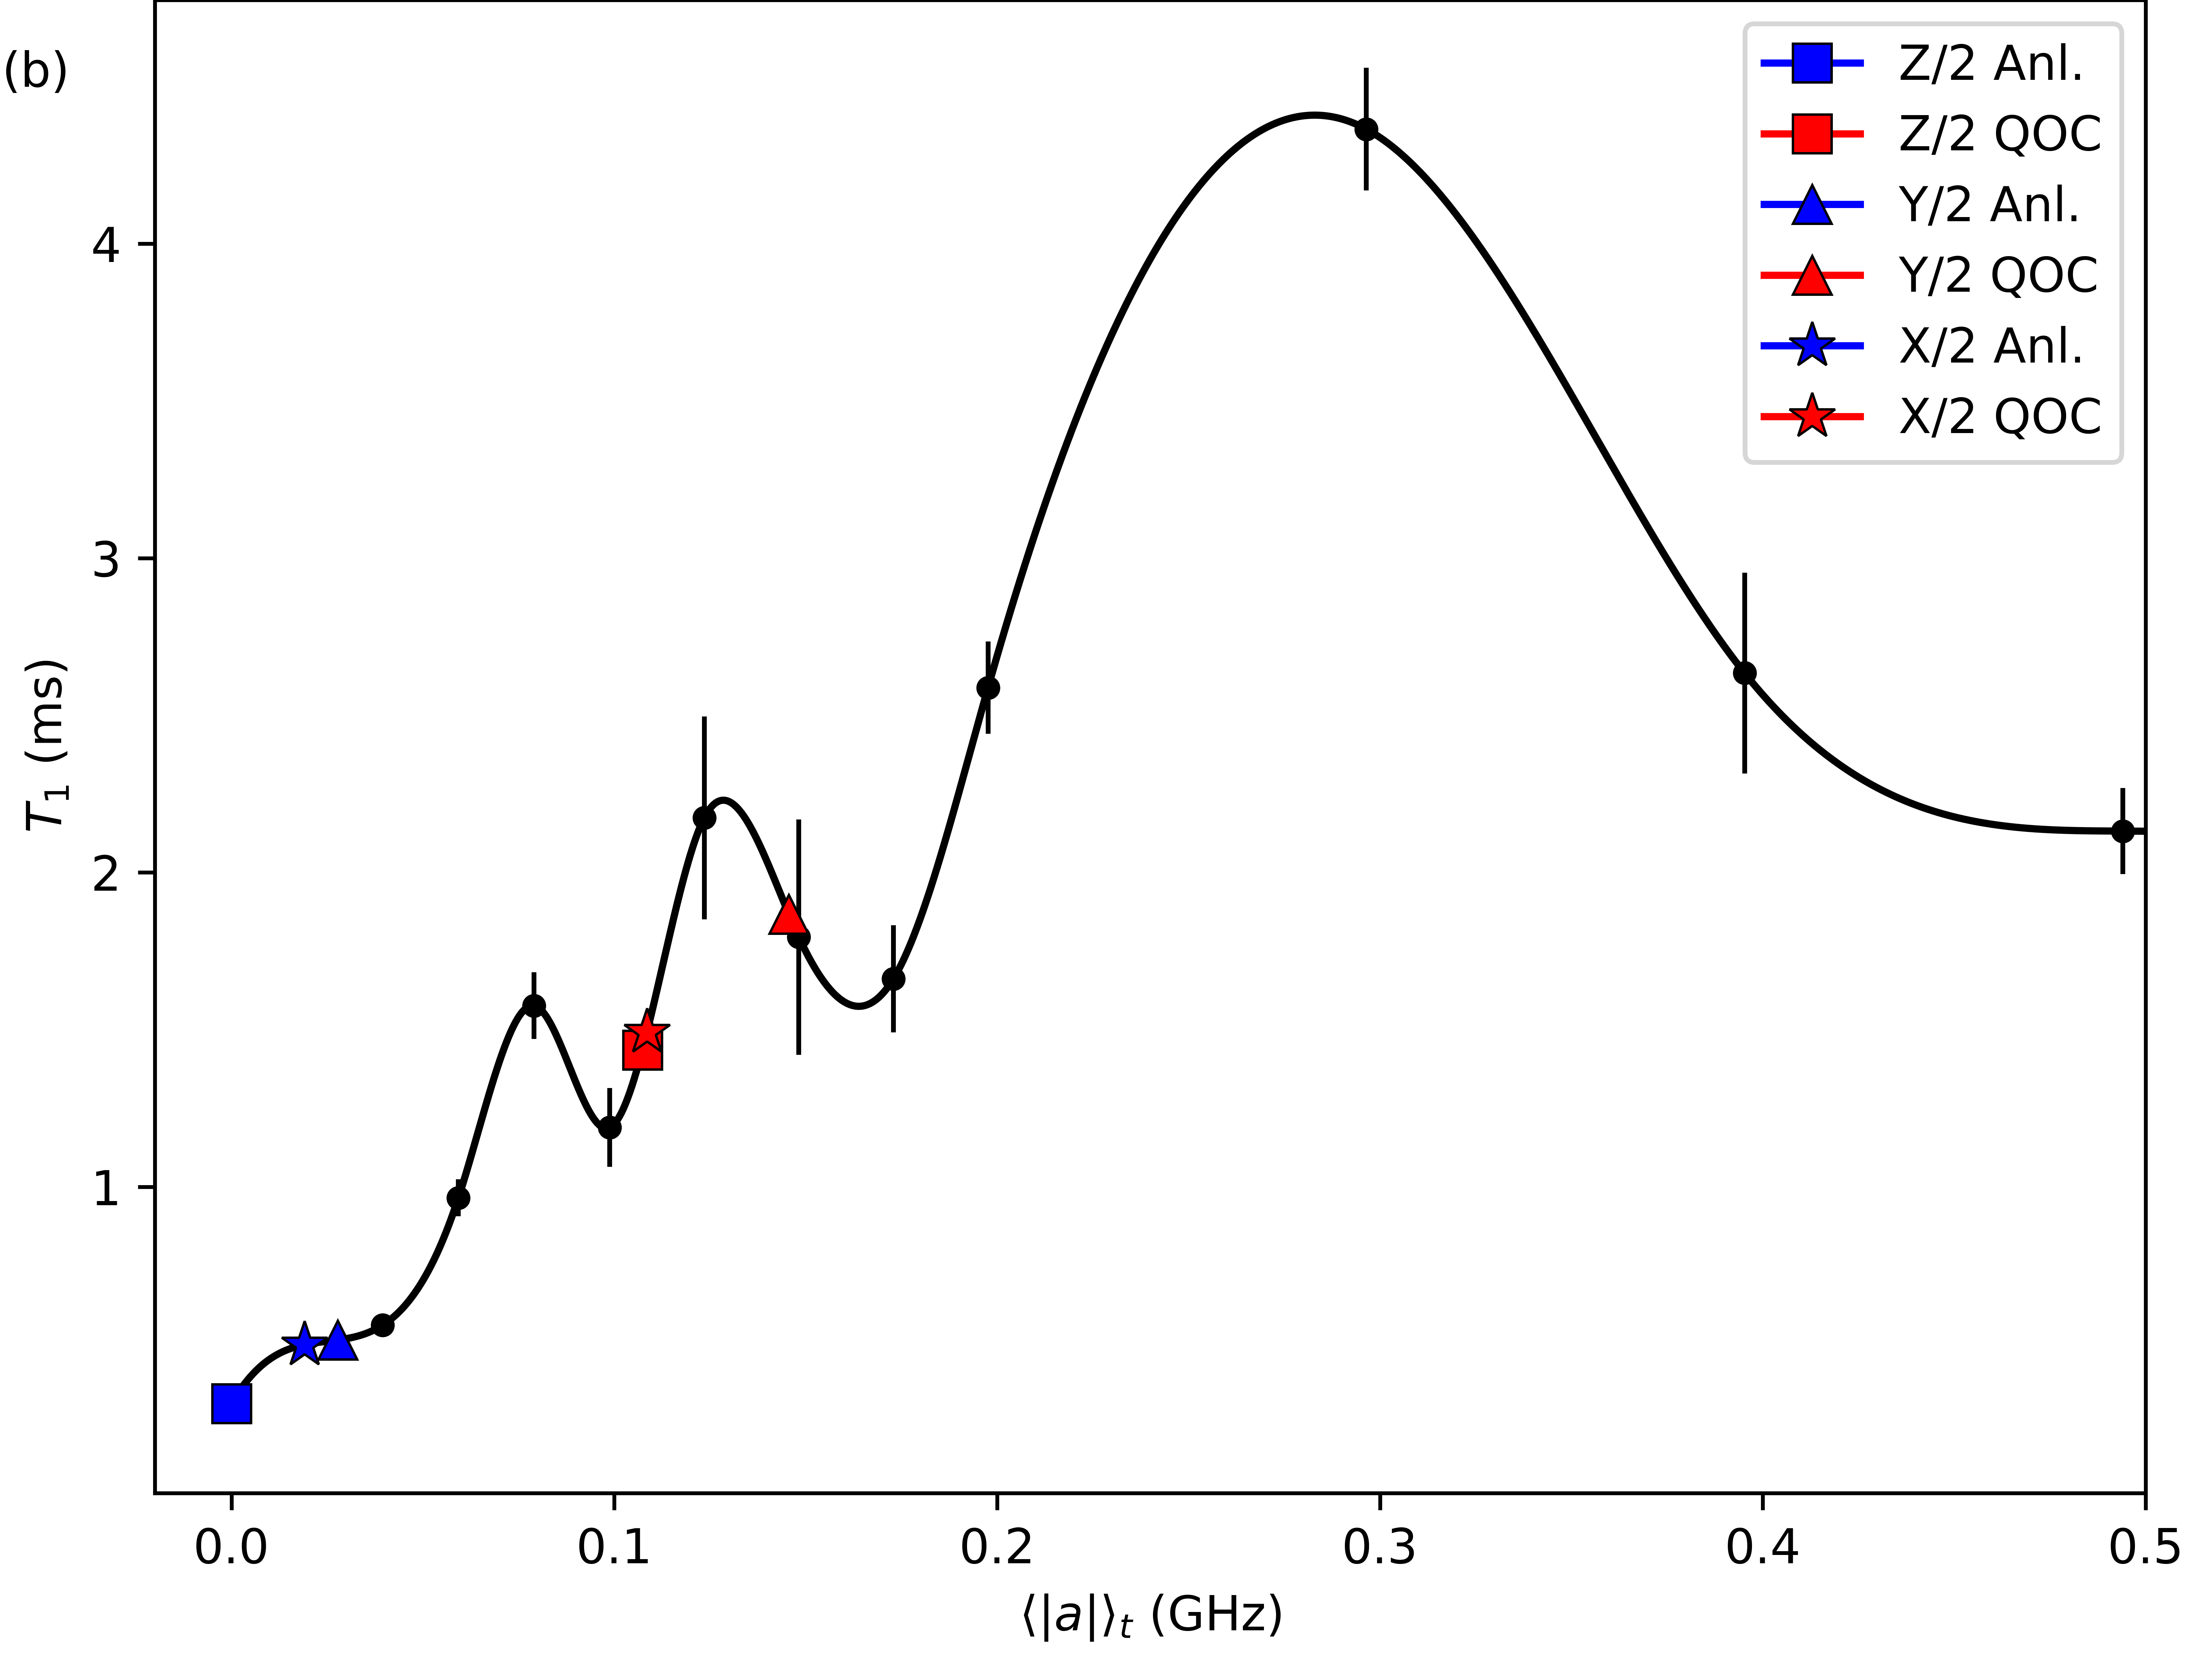
\includegraphics[width=\linewidth]{assets/f1b.png}
    \caption{\label{fig:longitudeb}}
  \end{subfigure}\hfill
  \begin{subfigure}{.4\textwidth}
    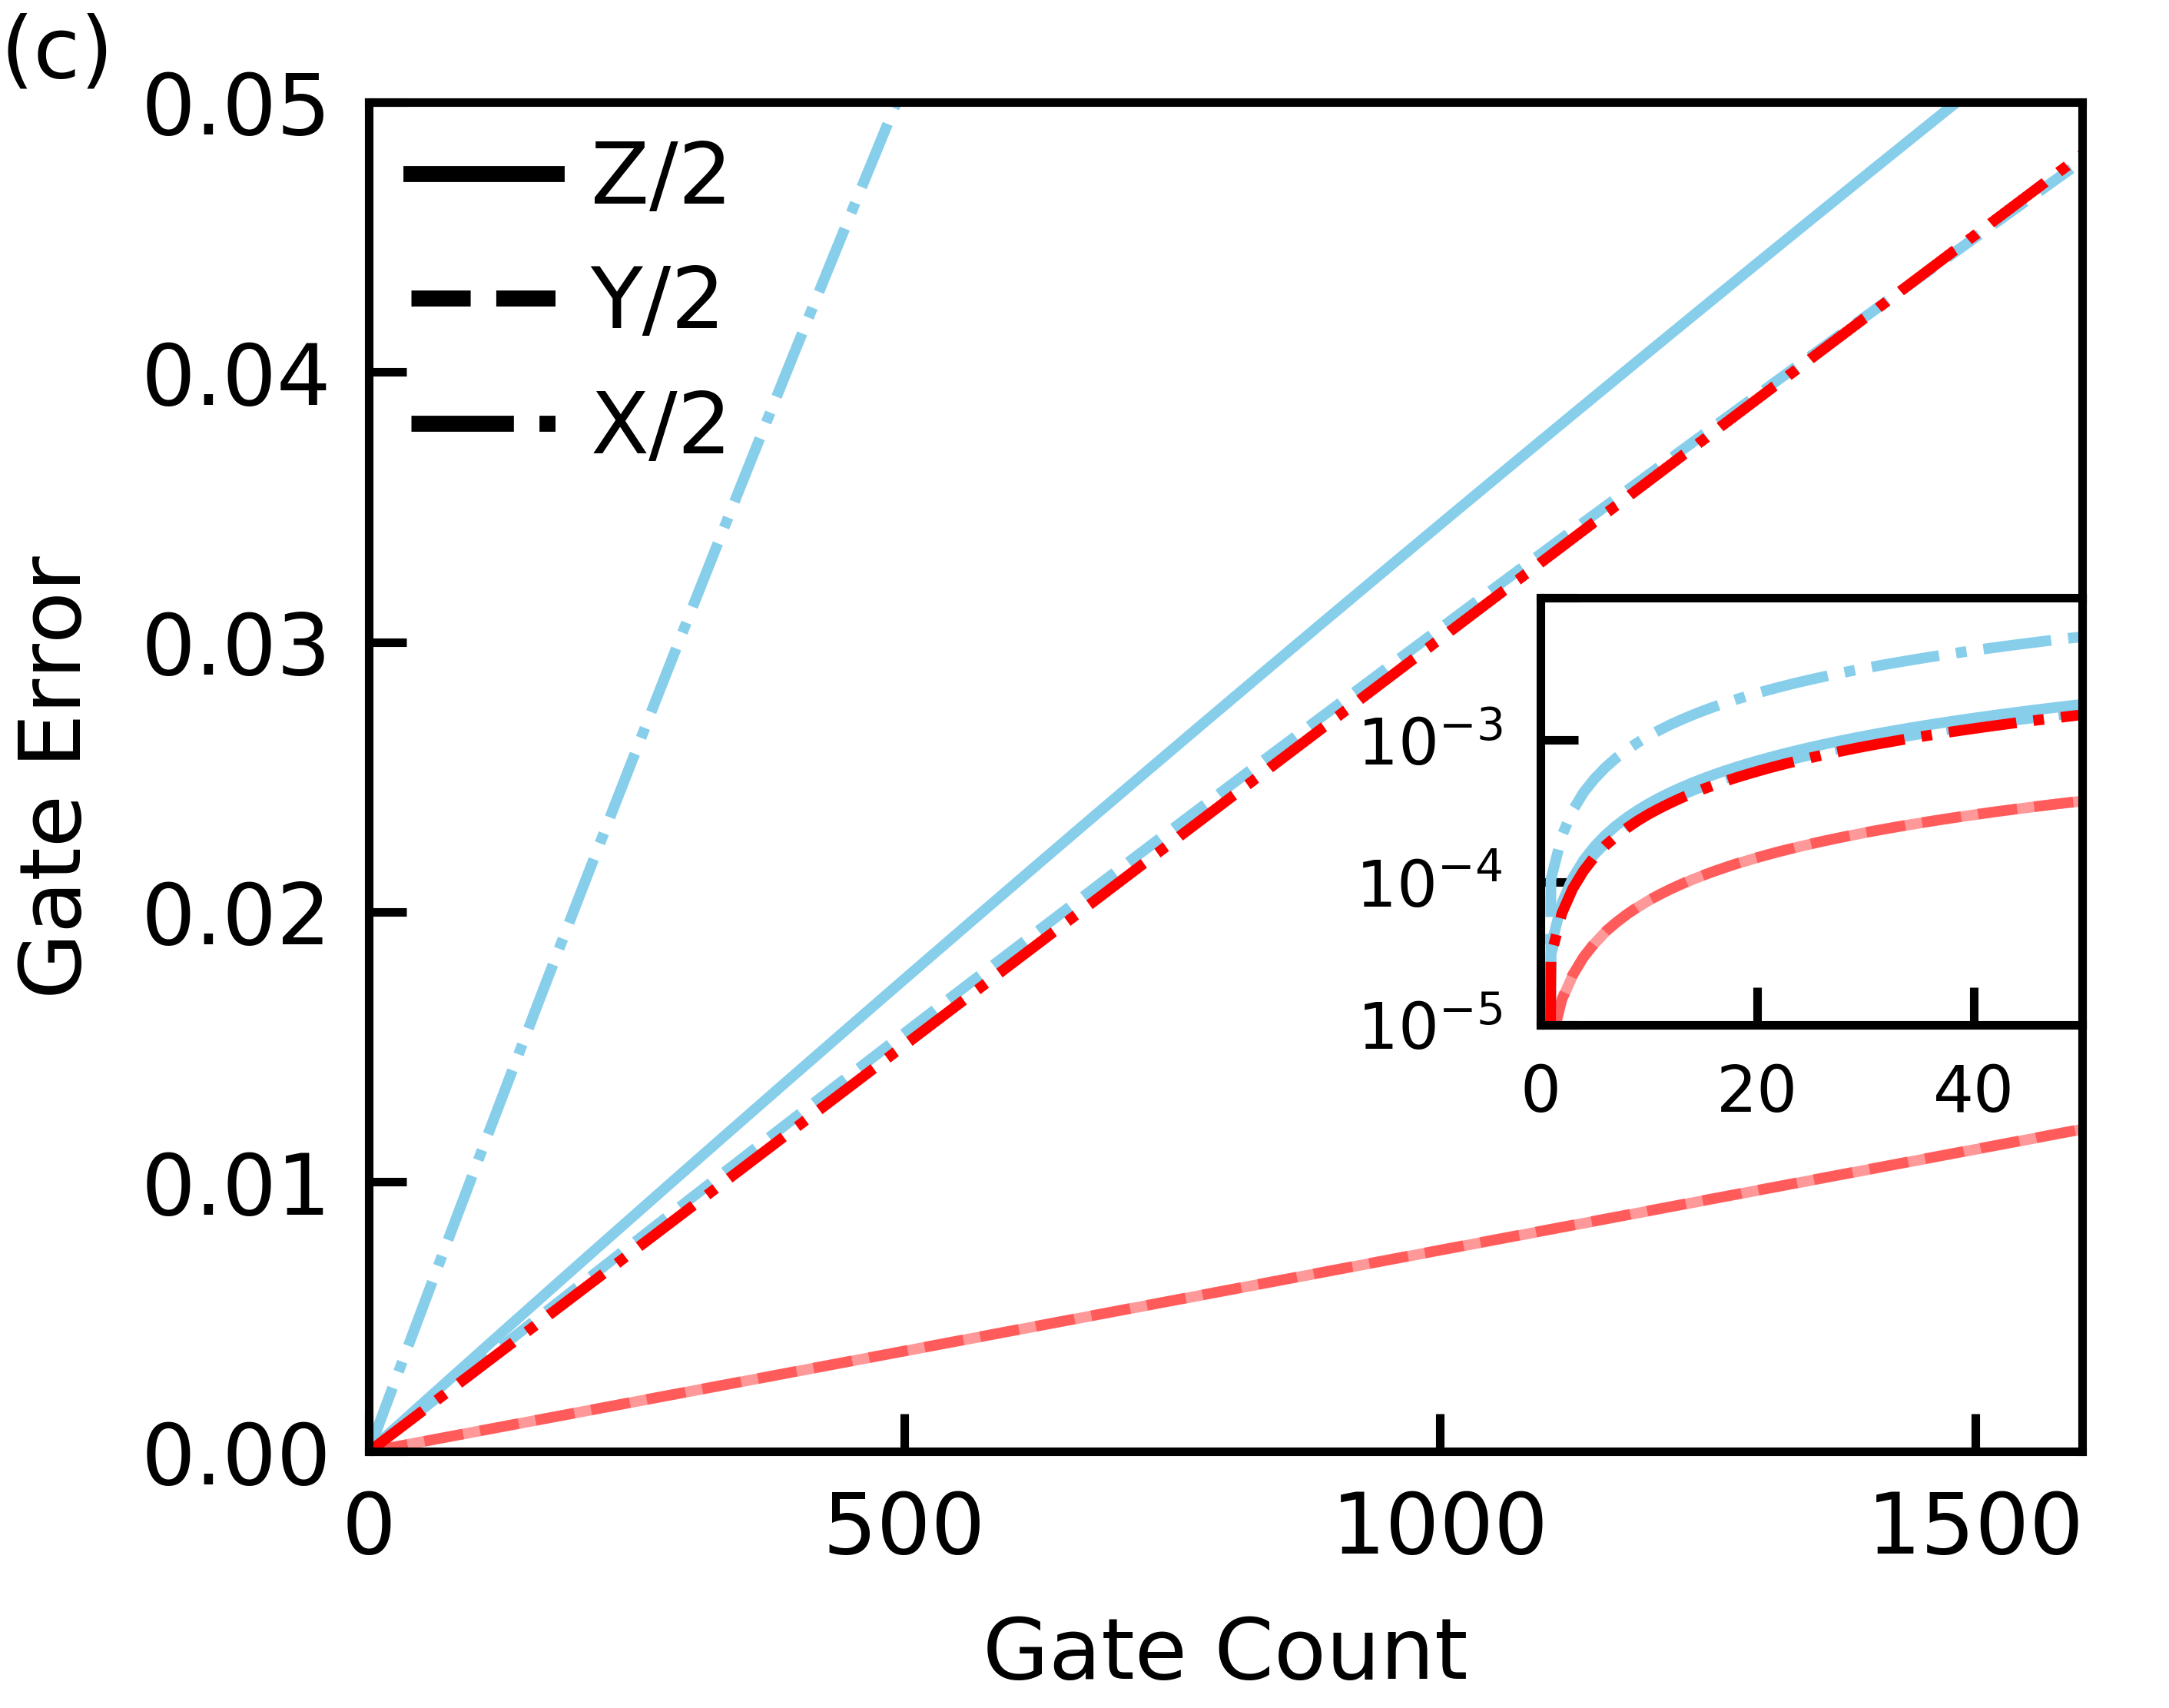
\includegraphics[width=\linewidth]{assets/f1c.png}
    \caption{\label{fig:longitudec}}
  \end{subfigure}
  \caption{
    (a) Flux pulses for the numerical gates (dark blue)
    and the analytic gates (light pink).
    (b) $T_{1}$ interpolation function used in optimization. Circle markers
    indicate measured $T_{1}$ times. Non-circle markers
    indicate the time-averaged, absolute amplitude of each flux pulse (seems a bit odd to plot these on this figure - it looks like you're assigning a T1 value to the entire pulse, which I'm not sure how to interpret).
    (c) Cumulative gate errors due to depolarization as a function of the
    number of gates applied.
    Cumulative gate errors for the numerical $Z/2$ and $Y/2$ gates
    are indistinguishable. Inset shows log-scaled cumulative gate errors
    for small gate counts.
  }
  \label{fig:longitude}
\end{figure*}

Next, we introduce the augmented control and augmented state:
\begin{equation}
  \begingroup
  \renewcommand*{\arraystretch}{1.3}
  u_{k} = \begin{bmatrix} \partial^{2}_{t} a_{k} \end{bmatrix}, \quad
  x_{k} = \begin{bmatrix} \ket{\psi^{0}_{k}} \\ \ket{\psi^{1}_{k}}
    \\ \int_{t} a_{k} \\ a_{k} \\ \partial_{t} a_{k} \end{bmatrix}.
  \endgroup
  \label{eq:astatecontrols}
\end{equation}
The variables in the augmented state are derived from
the decision variable in the augmented
control via coupled, first-order differential equations in the 
the discrete dynamics function \eqref{eq:dyn_con}.
We integrate the states according to the TDSE \eqref{eq:tdse} and the
fluxonium Hamiltonian \eqref{eq:hamiltonian} and integrate
the second-derivative of the flux amplitude to obtain
the first-derivative, proportional, and integral moments.
The ALTRO implementation we use does not currently
support complex numbers, so we repesent the states
in the isomorphism $\mathcal{H}(\mathbb{C}^{n})
\cong \mathcal{H}(\mathbb{R}^{2n})$ given in \cite{leung2017speedup},
\begin{equation}
  H \ket{\psi} \cong \begin{bmatrix} H_{\textrm{re}} & -H_{\textrm{im}}
    \\ H_{\textrm{im}} & H_{\textrm{re}}\end{bmatrix}
  \begin{bmatrix} \ket{\psi}_{\textrm{re}} \\ \ket{\psi}_{\textrm{im}}\end{bmatrix}.
  \label{eq:isomorphism}
\end{equation}
The cost function at each knot point is
$\ell_{k}(x_{k}, u_{k}) = (x_{k} - x_{f})^{T} Q_{k} (x_{k} - x_{f}) + u^{T}_{k} R_{k} u_{k}$
where $Q_{k}$ and $R_{k}$ are diagonal matrices we supply (didn't we say above that iLQR constructs quadratic models for each cost function? Is that what's going on here? How do we reconcile then that "we supply" Q and R?). The $Q_{k}$ term
penalizes deviations from the final augmented state $x_{f}$,
which is given by the constraints we have imposed on
$\ket*{\psi^{i}_{N}}$, $\int_{t} a_{N}$, and $a_{N}$ in addition to
$\partial_{t} a_{f} = 0$. The $R_{k}$ term penalizes the norm of $\partial^{2}_{t} a_{k}$,
mitigating AWG ringing due to high-frequency transitions.
Stated succinctly, the optimization problem takes the form:
\begin{mini!}[2] 
  {x_{1:N}, u_{1:N\text{-}1}}{\sum_{k=1}^N {(x_k\text{-}x_f)}^{T} Q_k (x_k\text{-}x_{f})
    + \sum_{k=1}^{N-1} {u_k}^{T} R_k u_{k}}{}{} \label{eq:costfun}
  \addConstraint{x_{k+1}}{= f(x_k, u_k)}  \label{eq:dyn_con}
  \addConstraint{\ket{\psi^{0}_{1}} = \ket{0}, \ket{\psi^{1}_{1}} = \ket{1}} \label{eq:istate_con}
  \addConstraint{\ket{\psi^{i}_{N}} = U \ket{\psi^{i}_{1}}
    \ \forall \  i} \label{eq:tstate_con}
  \addConstraint{{\lvert \braket{\psi^{i}_{k}}{\psi^{i}_{k}}
      \rvert}^{2} = 1 \ \forall \ i, k} \label{eq:statenorm_con}
  \addConstraint{{\textstyle \int_{t}} a_{N} = 0} \label{eq:znf_con}
  \addConstraint{|a_{k}| \leq 0.5 \ \textrm{GHz} \ \forall \ k} \label{eq:amp_con}
  \addConstraint{a_{1} = a_{N} = 0} \label{eq:bound_con}
  \addConstraint{{\textstyle \int_{t}} a_{1} = \partial_{t} a_{1} = 0}. \label{eq:ic_con}
\end{mini!}
